\documentclass[12pt]{article}
\usepackage[utf8]{inputenc}
\usepackage{graphicx}
\usepackage{subcaption}
\usepackage{amsmath}
\usepackage{fancyhdr}
\usepackage{geometry}
\usepackage{dirtytalk}
\usepackage[english]{babel}
\usepackage{csquotes}
\usepackage{hyperref}
\usepackage{listings}
\usepackage{xcolor}
\usepackage{booktabs}
\usepackage{longtable}
\usepackage{array}
\usepackage{tikz}
\usetikzlibrary{shapes.geometric, arrows, positioning, fit}
\usepackage[T1]{fontenc}

\lstset{
    language=C++,
    basicstyle=\ttfamily\small,
    numberstyle=\tiny,
    frame=single,
    breaklines=true,
    commentstyle=\color{green!50!black},
    keywordstyle=\color{blue},
    stringstyle=\color{red},
    showstringspaces=false,
    numbers=left
}

\linespread{1.25}
\setlength{\parindent}{0.8cm}
\setlength{\parskip}{0em}
\renewcommand{\headrulewidth}{0pt}
\geometry{a4paper, portrait, margin=1in}
\setlength{\headheight}{14.49998pt}
\graphicspath{{./}{../}}

% TikZ styles
\tikzstyle{startstop} = [rectangle, rounded corners, minimum width=3cm, minimum height=1cm, text centered, draw=black, fill=red!30]
\tikzstyle{process}   = [rectangle, minimum width=3.2cm, minimum height=1cm, text centered, draw=black, fill=blue!20]
\tikzstyle{decision}  = [diamond, minimum width=3.2cm, minimum height=1cm, text centered, draw=black, fill=green!20]
\tikzstyle{arrow}     = [thick,->,>=stealth]
\tikzstyle{block}     = [rectangle, draw, text width=7em, text centered, rounded corners, minimum height=3em]
\tikzset{every node/.style={align=center}}

% ============================================================================
\begin{document}

% ---------------------------------------------------------------------------
% TITLE PAGE
% ---------------------------------------------------------------------------
\begin{titlepage}
  \begin{center}
    \textsc{\large Ministry of Education of Republic of Moldova}\\[0.5cm]
    \textsc{\large Technical University of Moldova}\\[0.5cm]
    \textsc{\large Faculty of Computers, Informatics and Microelectronics}\\[0.5cm]
    \textsc{\large Software Engineering Department}\\[1.2cm]

    \vspace{20mm}
    \textsc{\Large Embedded Systems}\\[0.5cm]
    \textsc{\large Laboratory Work \#3}\\[0.5cm]

    \newcommand{\HRule}{\rule{\linewidth}{0.5mm}}
    \vspace{8mm}
    \HRule\\[0.4cm]
    {\LARGE \bfseries Button Duration Monitor with Multitasking\\[0.2cm]
    \large Bare-Metal Non-Preemptive Scheduling \& FreeRTOS\\[0.3cm]}
    \HRule\\[1.5cm]

    \begin{minipage}[t]{0.45\textwidth}
      \begin{flushleft}\large
        \emph{Author:}\\
        Sava \textsc{Luchian}\\
        std. gr. FAF-233
      \end{flushleft}
    \end{minipage}
    ~
    \begin{minipage}[t]{0.45\textwidth}
      \begin{flushright}\large
        \emph{Verified:}\\
        Alexei \textsc{Martiniuc}\\
      \end{flushright}
    \end{minipage}\\[2.5cm]

    \large Chisinau 2026
    \vfill
  \end{center}
\end{titlepage}

\setcounter{page}{2}
\pagestyle{fancy}
\fancyhf{}
\rhead{\thepage}
\lhead{FAF-233 Sava Luchian; Laboratory Work No.\ 3}

% ---------------------------------------------------------------------------
% TECHNICAL TASK
% ---------------------------------------------------------------------------
\section*{Technical Task}

\subsection*{Purpose of the Laboratory}
\hspace{0.8cm} Familiarise students with the fundamental concepts of embedded operating systems -- both bare-metal non-preemptive scheduling and FreeRTOS preemptive multitasking -- by implementing a button duration monitoring application that executes three concurrent tasks, demonstrates inter-task synchronisation, and reports periodic statistics via STDIO.

\subsection*{Objectives}
\begin{enumerate}
    \item Understand bare-metal non-preemptive task scheduling using timer interrupts, context structs, and recurrence/offset tables.
    \item Implement a FreeRTOS preemptive application with binary semaphores and mutexes.
    \item Port the same application logic between bare-metal and RTOS with minimal code changes.
    \item Demonstrate non-blocking task design (no busy-waiting) and safe shared-resource access.
    \item Validate system behaviour through Wokwi simulation and serial output analysis.
\end{enumerate}

\subsection*{Individual Task}
\hspace{0.8cm} Design and implement on an \textbf{Arduino Uno (ATmega328P)} a multitasking button monitoring application structured into at least three tasks:

\begin{itemize}
    \item \textbf{Task 1} -- Detect button press/release and measure press duration; signal \textbf{Green LED} for short press ($<$\,500\,ms) and \textbf{Red LED} for long press ($\geq$\,500\,ms).
    \item \textbf{Task 2} -- On each press: increment counters, accumulate duration statistics, and blink the \textbf{Yellow LED} (5$\times$ for short, 10$\times$ for long, 100\,ms period).
    \item \textbf{Task 3} -- Every 10\,s: print total presses, short/long counts, average durations via Serial, then reset all counters.
\end{itemize}

Implement the application twice: as a \textbf{Part 1} bare-metal sequential scheduler and as a \textbf{Part 2} FreeRTOS preemptive system.

% ---------------------------------------------------------------------------
% SECTION 1 â€`` DOMAIN ANALYSIS
% ---------------------------------------------------------------------------
\section{Domain Analysis}

\subsection{Technological Context and Application Domain}
\hspace{0.8cm} Multitasking is a foundational concept in embedded systems, enabling a single processor to interleave multiple logical activities efficiently. Embedded applications range from simple sensor-polling loops to safety-critical real-time systems that must respond to events within hard deadlines.

Two principal scheduling models exist in the field:

\begin{itemize}
    \item \textbf{Bare-metal non-preemptive (cooperative) scheduling}: The processor runs a single loop; tasks are short C functions invoked at regular intervals by a timer-driven dispatcher. No task can interrupt another. This model, popularised by automotive standards such as OSEK-VDX, is predictable, has zero context-switch overhead, and avoids concurrency hazards entirely.
    \item \textbf{Real-Time Operating System (RTOS) preemptive scheduling}: The kernel manages a set of independent tasks with their own stacks and can suspend the running task at any time to let a higher-priority task run. FreeRTOS is the leading open-source RTOS for microcontrollers, providing task creation, semaphores, mutexes, and queues.
\end{itemize}

This laboratory explores both models side-by-side on the same application to illustrate the trade-offs in complexity, resource usage, and correctness guarantees.

\subsection{Hardware Components and Justification}

\begin{table}[h!]
\centering
\begin{tabular}{p{4cm} p{2cm} p{7cm}}
\toprule
\textbf{Component} & \textbf{Qty} & \textbf{Role in the application} \\
\midrule
Arduino Uno (ATmega328P) & 1 & Main MCU; 16\,MHz, 2\,KB SRAM, 32\,KB Flash. Runs both bare-metal and FreeRTOS firmware. \\
Push-button & 1 & User input; one leg to D2, other to GND (INPUT\_PULLUP activated). \\
Green LED + 220\,$\Omega$ & 1 & Visual signal for short press ($<$\,500\,ms). \\
Red LED + 220\,$\Omega$ & 1 & Visual signal for long press ($\geq$\,500\,ms). \\
Yellow LED + 220\,$\Omega$ & 1 & Statistics blink feedback after each press. \\
Breadboard + jumper wires & -- & Prototyping interconnection. \\
USB cable & 1 & 5\,V power supply and serial communication. \\
\bottomrule
\end{tabular}
\caption{Hardware components used in Lab 3}
\label{tab:hardware}
\end{table}

The Arduino Uno was selected for its broad compatibility with PlatformIO, the feilipu/FreeRTOS AVR port, and the Wokwi hardware simulator, allowing rapid iteration without physical hardware.

\subsection{Software Components and Technologies}

\begin{itemize}
    \item \textbf{PlatformIO + VS Code}: Multi-environment project management. Two environments (\texttt{baremetal}, \texttt{freertos}) share the same source tree and use \texttt{build\_src\_filter} and \texttt{build\_flags} to select the active variant.
    \item \textbf{Arduino Framework (avr-arduino 5.2.0)}: GPIO abstractions (\texttt{pinMode}, \texttt{digitalWrite}), \texttt{Serial}, and the \texttt{millis()} timer.
    \item \textbf{AVR-libc}: Timer1 register access (\texttt{TCCR1A/B}, \texttt{OCR1A}, \texttt{TIMSK1}), ISR macro for bare-metal scheduling.
    \item \textbf{feilipu/FreeRTOS 11.1.0-3}: FreeRTOS kernel port for ATmega devices; provides task creation (\texttt{xTaskCreate}), binary semaphores (\texttt{xSemaphoreCreateBinary}), mutexes (\texttt{xSemaphoreCreateMutex}), and \texttt{vTaskDelayUntil}.
    \item \textbf{Wokwi Simulator}: Circuit + firmware simulation directly in VS Code; used for all functional testing.
\end{itemize}

\subsection{Analysis of Existing Solutions}
\hspace{0.8cm} Button debouncing and duration measurement are well-understood problems with established software patterns. The key design decision in this laboratory is the \emph{scheduling architecture}:

\begin{itemize}
    \item \textbf{Arduino \texttt{millis()}-based polling} (no scheduler): Simple but merges all logic into one \texttt{loop()}, becoming unmanageable above a few tasks.
    \item \textbf{TaskScheduler library}: Open-source cooperative scheduler for Arduino; comparable in concept to Part 1 but library-dependent.
    \item \textbf{FreeRTOS}: Industry-standard RTOS used in production embedded products (ESP-IDF, AWS IoT, motor controllers). Provides all required synchronisation primitives and deterministic task wakeup.
\end{itemize}

The chosen implementation follows the course theory: a hand-crafted bare-metal scheduler (Part 1) demonstrates the principles, then FreeRTOS (Part 2) replaces the manual machinery with proven OS infrastructure while keeping the application logic unchanged.

\subsection{Real-World Applications}
\hspace{0.8cm} Non-preemptive task scheduling and RTOS-based embedded multitasking appear across a wide range of commercial and industrial products:

\begin{itemize}
    \item \textbf{Industrial process controllers}: Use cooperative scheduling to sequence PLC-style operations with deterministic intervals and no complex synchronisation overhead. The producer-consumer task model used here mirrors standard IEC~61131 cyclic task concepts.
    \item \textbf{Automotive body control modules (BCM)}: OSEK/VDX-based non-preemptive kernels manage window, lock, and lighting tasks at fixed periods -- the same recurrence/offset dispatch pattern implemented in Part~1.
    \item \textbf{Battery-powered sensor nodes}: Cooperative schedulers minimise background CPU activity and allow deep-sleep between task periods, extending battery life. The 20\,ms polling cycle used for the button driver is a common IoT sensor pattern.
    \item \textbf{Medical device firmware}: Non-preemptive tasks with interrupt-only concurrency are favoured in safety-critical devices (IEC~62304) because their execution model is entirely auditable and testable without race-condition scenarios.
    \item \textbf{RTOS consumer electronics}: FreeRTOS runs in millions of IoT devices (ESP32, STM32-based products). The semaphore-driven event propagation from Task~1 to Task~2 mirrors the event-driven architecture of AWS IoT device SDKs built on FreeRTOS.
    \item \textbf{Home automation controllers}: Coordinate multiple peripherals (buttons, relays, sensors) using round-robin or priority task execution -- exactly the three-task pattern demonstrated here.
    \item \textbf{Motor controller firmware}: Use \texttt{vTaskDelayUntil}-style periodic tasks for current-control loops at fixed frequencies, and event semaphores for fault handling -- both patterns present in Part~2.
\end{itemize}

% ---------------------------------------------------------------------------
% SECTION 2 â€`` CONCEPTUALISATION AND DESIGN
% ---------------------------------------------------------------------------
\section{Conceptualisation and Design}

\subsection{Technical Requirements}

\begin{longtable}{p{1.5cm} p{2.5cm} p{7.5cm} p{1.5cm}}
\toprule
\textbf{ID} & \textbf{Category} & \textbf{Requirement} & \textbf{Type} \\
\midrule
\endfirsthead
R-F-01 & Button & System shall detect button press and release with software debounce (stable for $\geq$\,20\,ms). & Func. \\
R-F-02 & Button & System shall measure press duration in milliseconds from first stable press to first stable release. & Func. \\
R-F-03 & LED & Green LED shall illuminate for 800\,ms after a short press ($<$\,500\,ms) is detected. & Func. \\
R-F-04 & LED & Red LED shall illuminate for 800\,ms after a long press ($\geq$\,500\,ms) is detected. & Func. \\
R-F-05 & Statistics & System shall count total, short, and long presses independently and accumulate duration sums. & Func. \\
R-F-06 & LED & Yellow LED shall blink 5 times (100\,ms ON/OFF) after each short press. & Func. \\
R-F-07 & LED & Yellow LED shall blink 10 times (100\,ms ON/OFF) after each long press. & Func. \\
R-F-08 & Report & System shall print a statistics report to Serial every 10\,s: total, short, long counts and average durations. & Func. \\
R-F-09 & Report & System shall reset all counters to zero immediately after printing each report. & Func. \\
R-F-10 & Scheduling & Part 1 shall use a non-preemptive sequential scheduler driven by a 1\,ms Timer1 ISR. & Func. \\
R-F-11 & Scheduling & Part 2 shall use FreeRTOS preemptive tasks with binary semaphore and mutex synchronisation. & Func. \\
R-NF-01 & Latency & Maximum latency from button edge to LED response shall be $<$\,100\,ms. & Non-func. \\
R-NF-02 & CPU Load & CPU utilisation per system tick shall remain below 70\%. & Non-func. \\
R-NF-03 & Memory & Firmware shall fit within 32\,KB Flash and 2\,KB SRAM on the Arduino Uno. & Non-func. \\
R-NF-04 & Modularity & Application shall be structured in dedicated modules (config, peripherals, shared, os, tasks). & Non-func. \\
R-NF-05 & Portability & Core task logic shall be shared between bare-metal and FreeRTOS using conditional compilation only. & Non-func. \\
\bottomrule
\caption{Technical requirements for Lab 3}
\label{tab:requirements}
\end{longtable}

\subsection{Architectural Design}

\subsubsection{System Structural Architecture}

The application is divided into five software layers following the hardware--software boundary principle:

\begin{figure}[h!]
\centering
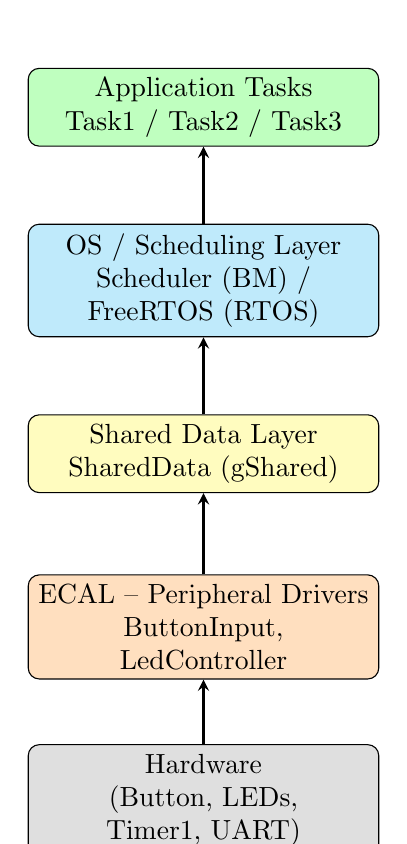
\begin{tikzpicture}
    \node (hw)     at (0, 0)   [block, fill=gray!25,   text width=12em, minimum height=2em]
          {Hardware\\(Button, LEDs, Timer1, UART)};
    \node (ecal)   at (0, 2.2) [block, fill=orange!25, text width=12em, minimum height=2em]
          {ECAL -- Peripheral Drivers\\ButtonInput, LedController};
    \node (shared) at (0, 4.4) [block, fill=yellow!25, text width=12em, minimum height=2em]
          {Shared Data Layer\\SharedData (gShared)};
    \node (sched)  at (0, 6.6) [block, fill=cyan!25,   text width=12em, minimum height=2em]
          {OS / Scheduling Layer\\Scheduler (BM) / FreeRTOS (RTOS)};
    \node (tasks)  at (0, 8.8) [block, fill=green!25,  text width=12em, minimum height=2em]
          {Application Tasks\\Task1 / Task2 / Task3};

    \draw [arrow] (hw)     -- (ecal);
    \draw [arrow] (ecal)   -- (shared);
    \draw [arrow] (shared) -- (sched);
    \draw [arrow] (sched)  -- (tasks);
\end{tikzpicture}
\caption{Layered software architecture}
\label{fig:layers}
\end{figure}

\subsubsection{HW/SW Interface and Component Interaction}

\begin{figure}[h!]
\centering
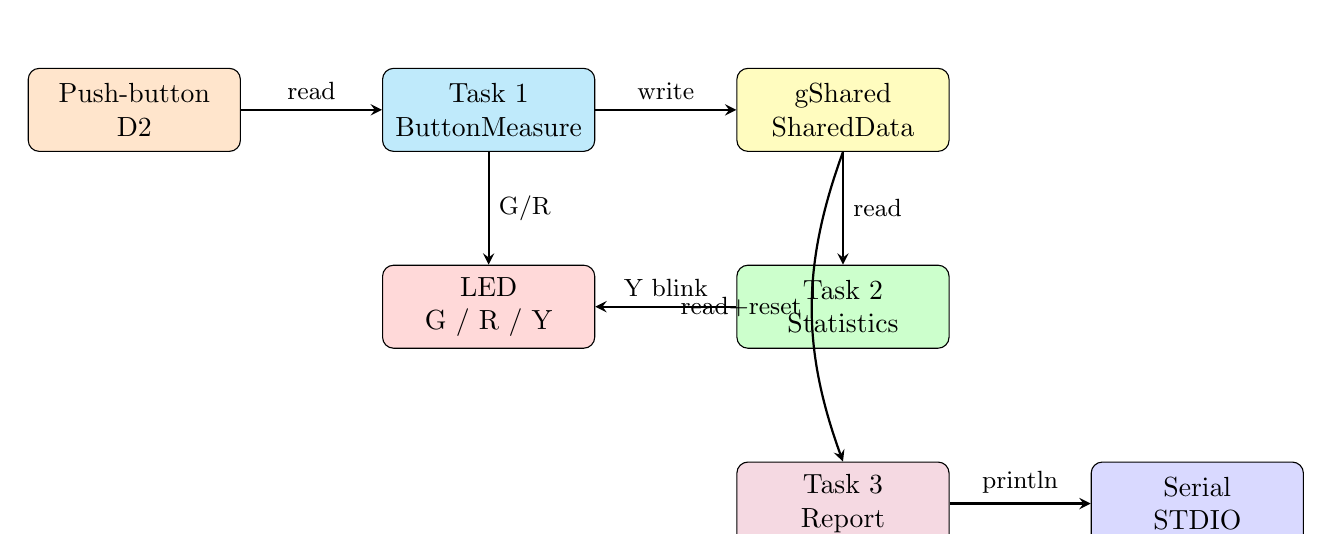
\begin{tikzpicture}
    % Row 1 (top): HW button  -->  Task1  -->  gShared
    \node (btn)     at (0,0)     [block, fill=orange!20] {Push-button\\D2};
    \node (task1)   at (4.5,0)   [block, fill=cyan!25]   {Task 1\\ButtonMeasure};
    \node (gshared) at (9.0,0)   [block, fill=yellow!25] {gShared\\SharedData};
    % Row 2: LEDs (below Task1)  and  Task2 (below gShared)
    \node (leds)    at (4.5,-2.5)[block, fill=red!15]    {LED\\G / R / Y};
    \node (task2)   at (9.0,-2.5)[block, fill=green!20]  {Task 2\\Statistics};
    % Row 3: Task3 (below Task2)  and  Serial (right of Task3)
    \node (task3)   at (9.0,-5.0)[block, fill=purple!15] {Task 3\\Report};
    \node (serial)  at (13.5,-5.0)[block, fill=blue!15]  {Serial\\STDIO};

    \draw [arrow] (btn)     -- node[above]{\small read}       (task1);
    \draw [arrow] (task1)   -- node[above]{\small write}      (gshared);
    \draw [arrow] (task1)   -- node[right]{\small G/R}        (leds);
    \draw [arrow] (gshared) -- node[right]{\small read}       (task2);
    \draw [arrow] (task2)   -- node[above]{\small Y blink}    (leds);
    \draw [arrow] (gshared.south) to[bend right=20] node[left]{\small read+reset} (task3.north);
    \draw [arrow] (task3)   -- node[above]{\small println}    (serial);
\end{tikzpicture}
\caption{Component interaction diagram}
\label{fig:interaction}
\end{figure}

\subsubsection{Bare-Metal Scheduler Design}

The scheduler follows the theory pattern exactly: a \texttt{Task\_t} struct holds a function pointer, recurrence, offset, and runtime countdown. Timer1 fires every 1\,ms in CTC mode; the ISR increments \texttt{sysTick\_ms} and sets a \texttt{tickFlag}. On each call to \texttt{os\_seq\_scheduler\_run()} from \texttt{loop()}, the flag is atomically cleared and all task counters are decremented. A task runs when its counter reaches zero, then the counter is reloaded with the recurrence value.

\begin{table}[h!]
\centering
\begin{tabular}{clrrl}
\toprule
\textbf{ID} & \textbf{Function} & \textbf{Period} & \textbf{Offset} & \textbf{Rationale} \\
\midrule
0 & \texttt{task\_button\_run} & 20\,ms & 0\,ms  & Debounce requires polling $\leq$\,20\,ms \\
1 & \texttt{task\_stats\_run}  & 20\,ms & 5\,ms  & Must execute after Task 1 (producer-first); staggered \\
2 & \texttt{task\_report\_run} & 10\,000\,ms & 10\,ms & Rare execution; negligible CPU load \\
\bottomrule
\end{tabular}
\caption{Bare-metal scheduler task table}
\label{tab:sched}
\end{table}

Priority is implicit in table order: Task\,0 is always dispatched before Task\,1 within the same tick, ensuring that button data is produced before statistics are consumed -- the \emph{producer-before-consumer} ordering from the theory.

\subsubsection{FreeRTOS Synchronisation Design}

\begin{table}[h!]
\centering
\begin{tabular}{llll}
\toprule
\textbf{Primitive} & \textbf{Name} & \textbf{Give (signal)} & \textbf{Take (wait)} \\
\midrule
Binary semaphore & \texttt{xButtonSemaphore} & Task 1 (after press) & Task 2 (event-driven) \\
Mutex & \texttt{xStatsMutex} & Any task releasing & Any task before accessing \texttt{gShared} \\
\bottomrule
\end{tabular}
\caption{FreeRTOS synchronisation primitives}
\label{tab:sync}
\end{table}

Task 2 blocks indefinitely on the binary semaphore (\texttt{portMAX\_DELAY}) -- consuming zero CPU while idle. This is the key advantage over the bare-metal polling approach. Task 3 uses \texttt{vTaskDelayUntil} for drift-free 10\,s wakeup regardless of its own execution time.

\subsection{Behavioural Modelling}

\subsubsection{ButtonInput Debounce FSM}

\begin{figure}[h!]
\centering
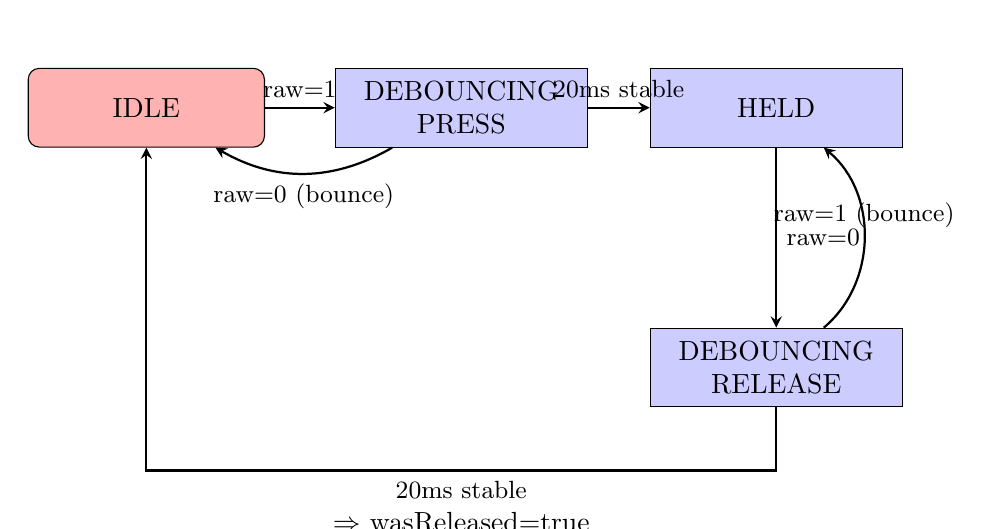
\begin{tikzpicture}[node distance=3cm, auto]
    \node[startstop] (idle)  {IDLE};
    \node[process]   (dp)    [right of=idle, xshift=1cm]  {DEBOUNCING\\PRESS};
    \node[process]   (held)  [right of=dp,   xshift=1cm]  {HELD};
    \node[process]   (dr)    [below of=held, yshift=-0.3cm] {DEBOUNCING\\RELEASE};

    \draw [arrow] (idle) -- node{\small raw=1} (dp);
    \draw [arrow] (dp)   to[bend left] node[below]{\small raw=0 (bounce)} (idle);
    \draw [arrow] (dp)   -- node{\small 20ms stable} (held);
    \draw [arrow] (held) -- node[right]{\small raw=0} (dr);
    \draw [arrow] (dr)   to[bend right=50] node[above]{\small raw=1 (bounce)} (held);
    \draw [arrow] (dr.south) -- ++(0,-0.8) -| node[pos=0.25,below]{\small 20ms stable\\$\Rightarrow$ wasReleased=true} (idle.south);
\end{tikzpicture}
\caption{ButtonInput debounce finite-state machine}
\label{fig:button-fsm}
\end{figure}

\subsubsection{Task 1 Flowchart}

\begin{figure}[h!]
\centering
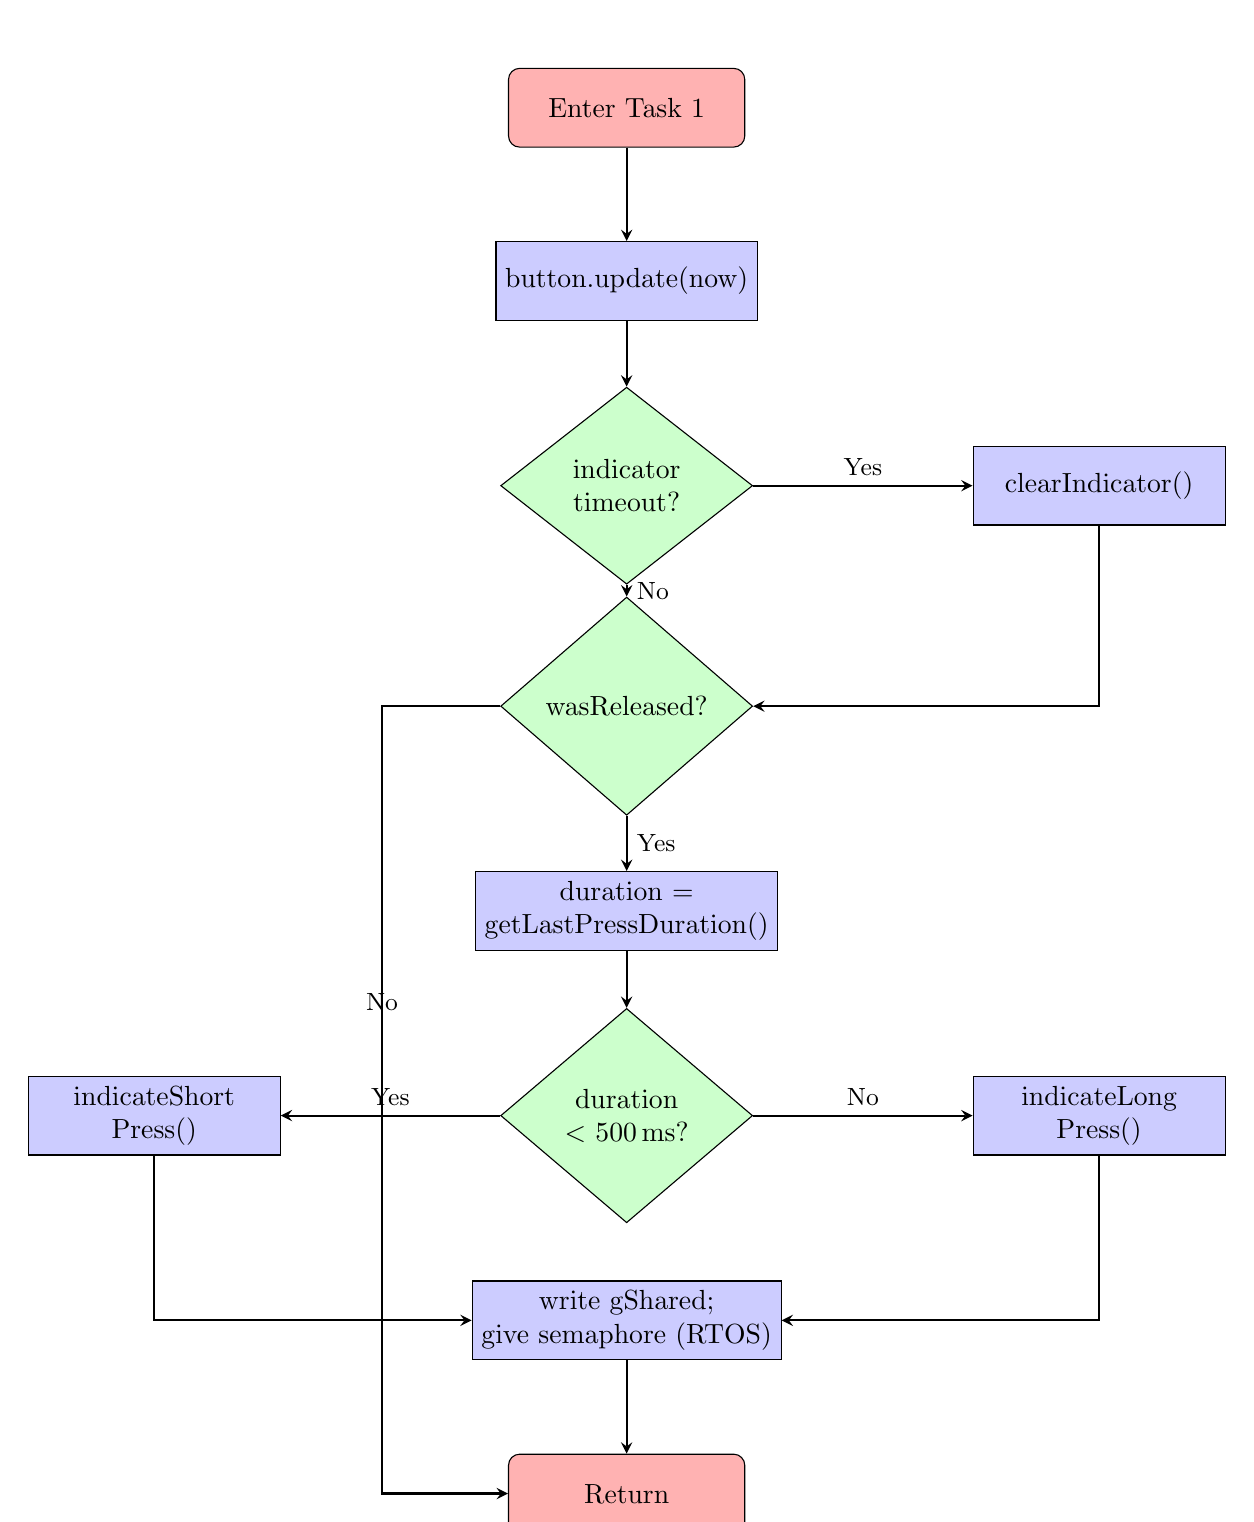
\begin{tikzpicture}
    \node (s)   at ( 0,    0)    [startstop] {Enter Task 1};
    \node (upd) at ( 0,   -2.2)  [process]   {button.update(now)};
    \node (led) at ( 0,   -4.8)  [decision]  {indicator\\timeout?};
    \node (clr) at ( 6.0, -4.8)  [process]   {clearIndicator()};
    \node (rel) at ( 0,   -7.6)  [decision]  {wasReleased?};
    \node (dur) at ( 0,   -10.2) [process]   {duration =\\getLastPressDuration()};
    \node (sht) at ( 0,   -12.8) [decision]  {duration\\$<$ 500\,ms?};
    \node (grn) at (-6.0, -12.8) [process]   {indicateShort\\Press()};
    \node (red) at ( 6.0, -12.8) [process]   {indicateLong\\Press()};
    \node (pub) at ( 0,   -15.4) [process]   {write gShared;\\give semaphore (RTOS)};
    \node (ret) at ( 0,   -17.6) [startstop] {Return};

    \draw [arrow] (s)   -- (upd);
    \draw [arrow] (upd) -- (led);
    \draw [arrow] (led) -- node[above]{\small Yes} (clr);
    \draw [arrow] (clr.south) |- (rel.east);
    \draw [arrow] (led) -- node[right]{\small No}  (rel);
    \draw [arrow] (rel) -- node[right]{\small Yes} (dur);
    \draw [arrow] (rel.west) -- ++(-1.5,0) |- node[pos=0.2,above]{\small No} (ret.west);
    \draw [arrow] (dur) -- (sht);
    \draw [arrow] (sht) -- node[above]{\small Yes} (grn);
    \draw [arrow] (sht) -- node[above]{\small No}  (red);
    \draw [arrow] (grn.south) |- (pub.west);
    \draw [arrow] (red.south) |- (pub.east);
    \draw [arrow] (pub) -- (ret);
\end{tikzpicture}
\caption{Task 1 flowchart -- button detection and LED signalling}
\label{fig:task1flow}
\end{figure}

\subsubsection{Task 2 Flowchart}

\begin{figure}[h!]
\centering
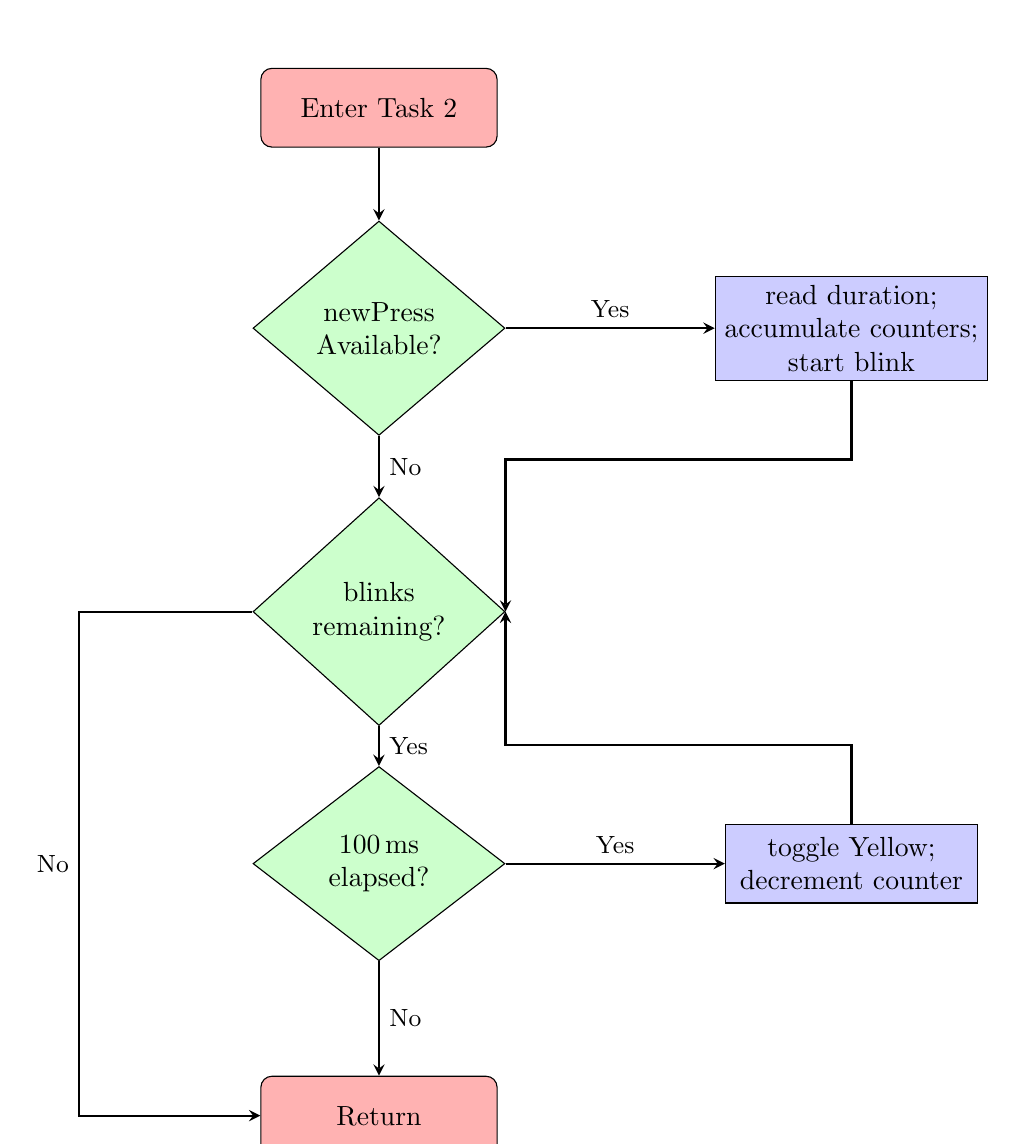
\begin{tikzpicture}
    \node (s)   at (0,    0)    [startstop] {Enter Task 2};
    \node (npa) at (0,   -2.8)  [decision]  {newPress\\Available?};
    \node (clr) at (6.0, -2.8)  [process]   {read duration;\\accumulate counters;\\start blink};
    \node (bl)  at (0,   -6.4)  [decision]  {blinks\\remaining?};
    \node (tog) at (0,   -9.6)  [decision]  {100\,ms\\elapsed?};
    \node (tgl) at (6.0, -9.6)  [process]   {toggle Yellow;\\decrement counter};
    \node (ret) at (0,  -12.8)  [startstop] {Return};

    \draw [arrow] (s)   -- (npa);
    % Yes: npa -> clr -> back to bl from above-right
    \draw [arrow] (npa) -- node[above]{\small Yes} (clr);
    \draw [arrow] (clr.south) -- ++(0,-1.0) -| (bl.east);
    % No: npa -> bl straight down
    \draw [arrow] (npa) -- node[right]{\small No}  (bl);
    % No from bl: exit LEFT, bypass tog, arrive at ret from left
    \draw [arrow] (bl.west) -- ++(-2.2,0) |- node[pos=0.25,left]{\small No} (ret.west);
    % Yes from bl: down to tog
    \draw [arrow] (bl)  -- node[right]{\small Yes} (tog);
    % No from tog: straight down to ret
    \draw [arrow] (tog) -- node[right]{\small No}  (ret);
    % Yes from tog: right to tgl, then tgl loops back up to bl from right
    \draw [arrow] (tog) -- node[above]{\small Yes} (tgl);
    \draw [arrow] (tgl.north) -- ++(0,1.0) -| (bl.east);
\end{tikzpicture}
\caption{Task 2 flowchart -- statistics and non-blocking yellow LED blink (bare-metal)}
\label{fig:task2flow}
\end{figure}

\subsubsection{Task 3 Flowchart}

\begin{figure}[h!]
\centering
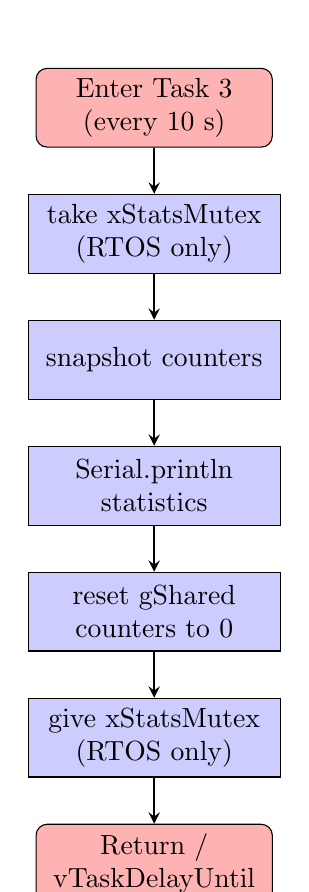
\begin{tikzpicture}[node distance=1.6cm]
    \node (s)   [startstop] {Enter Task 3\\(every 10 s)};
    \node (mtx) [process, below of=s] {take xStatsMutex\\(RTOS only)};
    \node (snap)[process, below of=mtx] {snapshot counters};
    \node (prt) [process, below of=snap] {Serial.println\\statistics};
    \node (rst) [process, below of=prt] {reset gShared\\counters to 0};
    \node (rel) [process, below of=rst] {give xStatsMutex\\(RTOS only)};
    \node (ret) [startstop, below of=rel] {Return /\\vTaskDelayUntil};

    \draw [arrow] (s) -- (mtx);
    \draw [arrow] (mtx) -- (snap);
    \draw [arrow] (snap) -- (prt);
    \draw [arrow] (prt) -- (rst);
    \draw [arrow] (rst) -- (rel);
    \draw [arrow] (rel) -- (ret);
\end{tikzpicture}
\caption{Task 3 flowchart -- periodic STDIO report}
\label{fig:task3flow}
\end{figure}

\subsubsection{Timing Diagram (Bare-Metal Scheduler)}

The diagram below visualises task execution slots over the first 120\,ms of operation. Task~0 fires at $t=0, 20, 40 \ldots$ ms; Task~1 fires at $t=5, 25, 45 \ldots$ ms (5\,ms offset); Task~2 first fires at $t=10\,000$\,ms and is not visible in this window.

\begin{figure}[htbp]
\centering
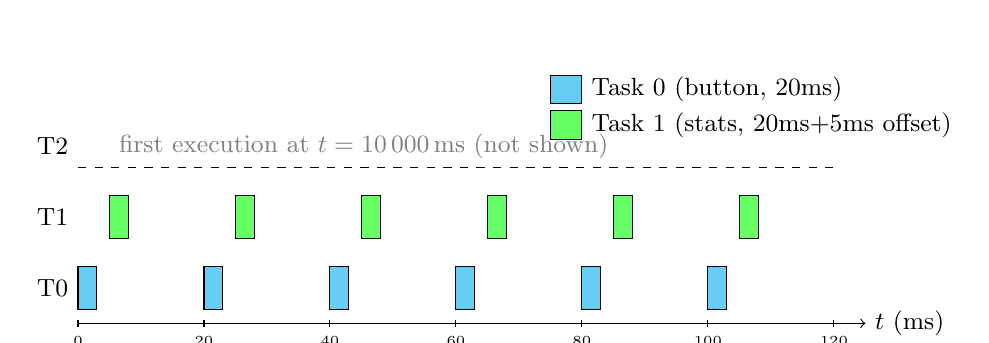
\begin{tikzpicture}[x=0.08cm, y=0.9cm]
  % Axis
  \draw[->] (0,0) -- (125,0) node[right]{\small $t$ (ms)};
  \foreach \x in {0,20,40,60,80,100,120}
      \draw (\x,0.05) -- (\x,-0.05) node[below]{\tiny \x};
  % Task 0 bars (period=20, offset=0, width~3ms)
  \foreach \s in {0,20,40,60,80,100}
      \filldraw[fill=cyan!60,draw=black] (\s,0.2) rectangle (\s+3,0.8);
  \node[left] at (0,0.5) {\small T0};
  % Task 1 bars (period=20, offset=5, width~3ms)
  \foreach \s in {5,25,45,65,85,105}
      \filldraw[fill=green!60,draw=black] (\s,1.2) rectangle (\s+3,1.8);
  \node[left] at (0,1.5) {\small T1};
  % Task 2 label only (period=10000, won't appear)
  \node[left] at (0,2.5) {\small T2};
  \draw[dashed] (0,2.2) -- (120,2.2);
  \node[right,gray] at (5,2.5) {\small first execution at $t=10\,000$\,ms (not shown)};
  % Legend
  \filldraw[fill=cyan!60] (75,3.1) rectangle (80,3.5); \node[right] at (80,3.3){\small Task~0 (button, 20ms)};
  \filldraw[fill=green!60] (75,2.6) rectangle (80,3.0); \node[right] at (80,2.8){\small Task~1 (stats, 20ms+5ms offset)};
\end{tikzpicture}
\caption{Bare-metal task execution timing over first 120\,ms}
\label{fig:timing}
\end{figure}

The 5\,ms offset between Task~0 and Task~1 guarantees that within the same 20\,ms window the button data is always written before statistics are read -- the non-preemptive producer-before-consumer guarantee. No two tasks execute simultaneously, eliminating all intra-tick race conditions.

\subsubsection{Sequence Diagram}

The sequence diagram below shows the complete inter-task communication flow triggered by a single button press event.

\begin{figure}[htbp]
\centering
\resizebox{\textwidth}{!}{%
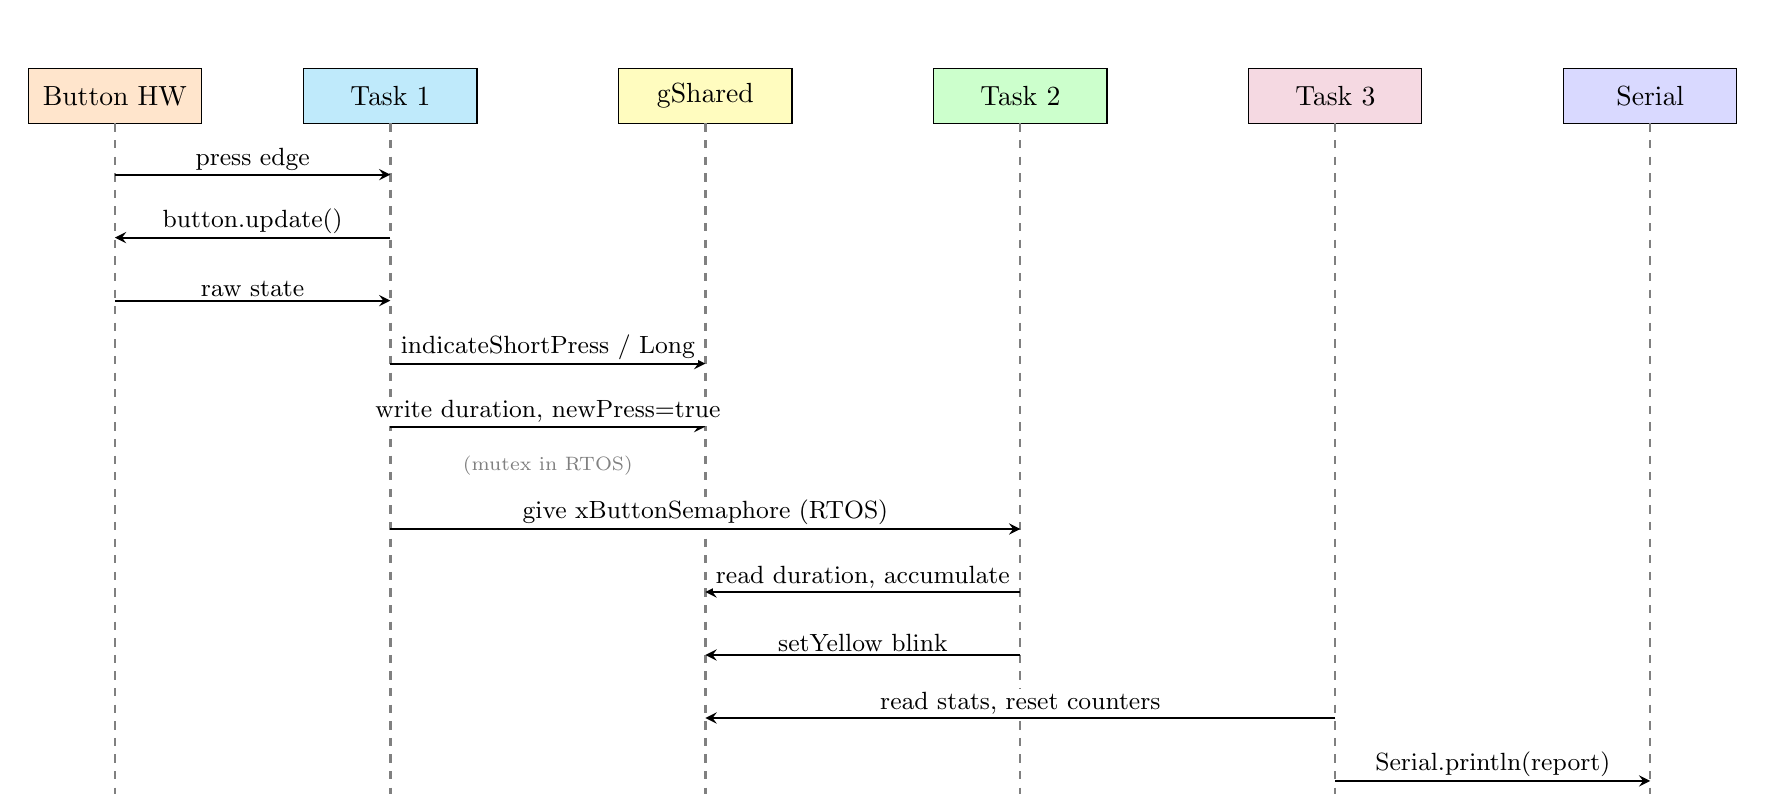
\begin{tikzpicture}[
    lifeline/.style={thick},
    msg/.style={->,>=stealth,thick},
    lbl/.style={font=\small,fill=white,inner sep=1pt}
]
  % Lifeline headers
  \node (HW)   at (0,   0) [draw, fill=orange!20, minimum width=2.2cm, minimum height=0.7cm] {Button HW};
  \node (T1)   at (3.5, 0) [draw, fill=cyan!25,   minimum width=2.2cm, minimum height=0.7cm] {Task 1};
  \node (SH)   at (7.5, 0) [draw, fill=yellow!25, minimum width=2.2cm, minimum height=0.7cm] {gShared};
  \node (T2)   at (11.5,0) [draw, fill=green!20,  minimum width=2.2cm, minimum height=0.7cm] {Task 2};
  \node (T3)   at (15.5,0) [draw, fill=purple!15, minimum width=2.2cm, minimum height=0.7cm] {Task 3};
  \node (SER)  at (19.5,0) [draw, fill=blue!15,   minimum width=2.2cm, minimum height=0.7cm] {Serial};
  % Lifelines
  \foreach \x in {0,3.5,7.5,11.5,15.5,19.5}
      \draw[lifeline,dashed,gray] (\x,-0.35) -- (\x,-9.0);
  % Messages
  \draw[msg] (0,-1.0)   -- node[lbl,above]{press edge}                    (3.5,-1.0);
  \draw[msg] (3.5,-1.8) -- node[lbl,above]{button.update()}               (0,-1.8);
  \draw[msg] (0,-2.6)   -- node[lbl,above]{raw state}                     (3.5,-2.6);
  \draw[msg] (3.5,-3.4) -- node[lbl,above]{indicateShortPress / Long}     (7.5,-3.4);
  \draw[msg] (3.5,-4.2) -- node[lbl,above]{write duration, newPress=true} (7.5,-4.2);
  \node[font=\scriptsize,gray] at (5.5,-4.7) {(mutex in RTOS)};
  \draw[msg] (3.5,-5.5) -- node[lbl,above]{give xButtonSemaphore (RTOS)} (11.5,-5.5);
  \draw[msg] (11.5,-6.3)-- node[lbl,above]{read duration, accumulate}    (7.5,-6.3);
  \draw[msg] (11.5,-7.1)-- node[lbl,above]{setYellow blink}              (7.5,-7.1);
  \draw[msg] (15.5,-7.9)-- node[lbl,above]{read stats, reset counters}   (7.5,-7.9);
  \draw[msg] (15.5,-8.7)-- node[lbl,above]{Serial.println(report)}       (19.5,-8.7);
\end{tikzpicture}%
}%
\caption{Sequence diagram -- inter-task communication on button press}
\label{fig:sequence}
\end{figure}

The unidirectional data flow (Task~1 $\rightarrow$ \texttt{gShared} $\rightarrow$ Task~2/Task~3) prevents circular dependencies. In bare-metal mode, \texttt{newPressAvailable} is a simple volatile flag cleared atomically; in FreeRTOS mode the binary semaphore replaces it, providing a blocking wait instead of polling.

\subsubsection{Full System State Machine}

The complete state machine below unifies the scheduler state and all three task internal states, matching the behaviour described in the implementation.

\begin{figure}[htbp]
\centering
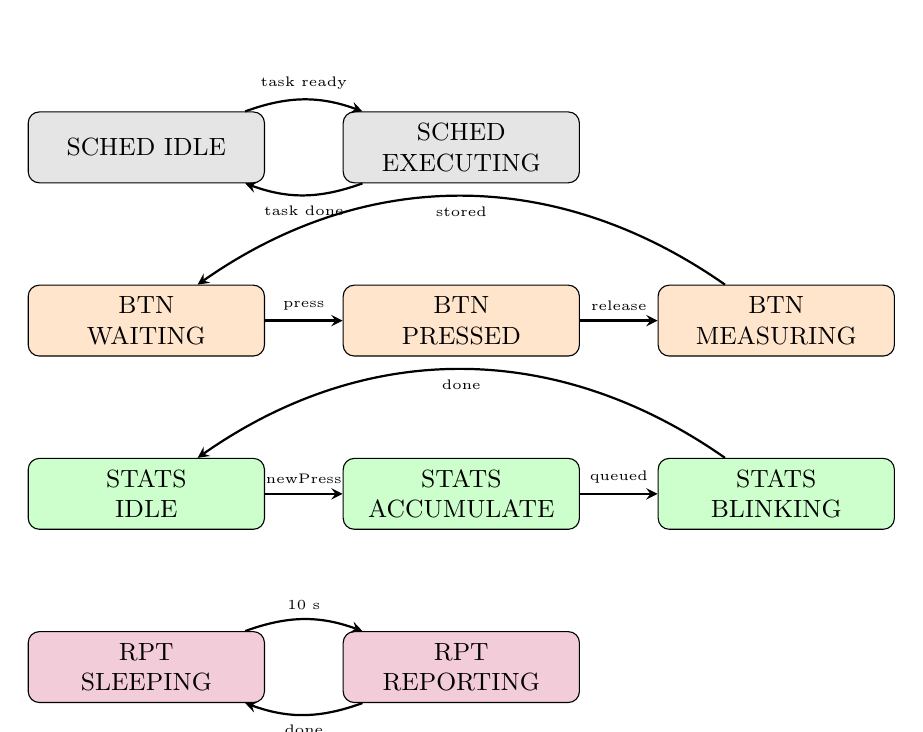
\begin{tikzpicture}[
    state/.style={rectangle, rounded corners, draw, fill=blue!12,
                  minimum width=3.0cm, minimum height=0.9cm, font=\small}
]
  % --- Scheduler group (row 1) ---
  \node[state, fill=gray!20]   (SIDLE) at (0,    0)   {SCHED IDLE};
  \node[state, fill=gray!20]   (SEXEC) at (4.0,  0)   {SCHED\\EXECUTING};
  \draw[arrow] (SIDLE) to[bend left=20]  node[above]{\tiny task ready} (SEXEC);
  \draw[arrow] (SEXEC) to[bend left=20]  node[below]{\tiny task done}  (SIDLE);

  % --- Button FSM group (row 2) ---
  \node[state, fill=orange!20] (BW) at (0,   -2.2) {BTN\\WAITING};
  \node[state, fill=orange!20] (BP) at (4.0, -2.2) {BTN\\PRESSED};
  \node[state, fill=orange!20] (BM) at (8.0, -2.2) {BTN\\MEASURING};
  \draw[arrow] (BW) -- node[above]{\tiny press}   (BP);
  \draw[arrow] (BP) -- node[above]{\tiny release} (BM);
  \draw[arrow] (BM) to[bend right=35] node[below]{\tiny stored} (BW);

  % --- Stats task group (row 3) ---
  \node[state, fill=green!20]  (STID)  at (0,   -4.4) {STATS\\IDLE};
  \node[state, fill=green!20]  (STACC) at (4.0, -4.4) {STATS\\ACCUMULATE};
  \node[state, fill=green!20]  (STBL)  at (8.0, -4.4) {STATS\\BLINKING};
  \draw[arrow] (STID)  -- node[above]{\tiny newPress} (STACC);
  \draw[arrow] (STACC) -- node[above]{\tiny queued}   (STBL);
  \draw[arrow] (STBL)  to[bend right=35] node[below]{\tiny done} (STID);

  % --- Report task group (row 4) ---
  \node[state, fill=purple!20] (RSLP) at (0,   -6.6) {RPT\\SLEEPING};
  \node[state, fill=purple!20] (RRPT) at (4.0, -6.6) {RPT\\REPORTING};
  \draw[arrow] (RSLP) to[bend left=20]  node[above]{\tiny 10 s} (RRPT);
  \draw[arrow] (RRPT) to[bend left=20]  node[below]{\tiny done} (RSLP);
\end{tikzpicture}
\caption{Full system state machine -- scheduler and all task states}
\label{fig:fsm-full}
\end{figure}

The scheduler oscillates between IDLE (no task period elapsed) and EXECUTING (one task running to completion). The button driver transitions through four states tracking press stability. The statistics task starts idle, accumulates on a new press event, then drives the blink sequence. The report task sleeps for 10\,s then wakes to print and reset before returning to sleep.

\subsection{Test Scenarios and Validation Criteria}

\begin{longtable}{p{1.0cm} p{2.3cm} p{4.5cm} p{4.5cm} p{1.0cm}}
\toprule
\textbf{ID} & \textbf{Category} & \textbf{Scenario} & \textbf{Expected result} & \textbf{Req.} \\
\midrule
\endfirsthead
T-01 & Button & Press button for $\approx$\,200\,ms then release & Green LED turns ON within 20\,ms; stays ON 800\,ms & R-F-01..03 \\
T-02 & Button & Press button for $\approx$\,1\,000\,ms then release & Red LED turns ON within 20\,ms; stays ON 800\,ms & R-F-01..02, R-F-04 \\
T-03 & LED blink & Short press executed & Yellow LED blinks exactly 5 times at 100\,ms intervals & R-F-06 \\
T-04 & LED blink & Long press executed & Yellow LED blinks exactly 10 times at 100\,ms intervals & R-F-07 \\
T-05 & Statistics & 3 short + 2 long in one 10\,s window & Serial report: total=5, short=3, long=2; averages computed correctly & R-F-05, R-F-08 \\
T-06 & Reset & After report printed & Next 10\,s window starts from all counters = 0 & R-F-09 \\
T-07 & Idle & No presses in 10\,s & Report shows total=0, no division-by-zero on averages & R-F-08 \\
T-08 & Debounce & Rapid button contact noise ($<$\,20\,ms) & No press registered; counters unchanged & R-F-01 \\
T-09 & Concurrency & FreeRTOS: Task 2 blinks while Task 3 reports simultaneously & Counters consistent; no corruption & R-F-11 \\
T-10 & Latency & Time from button press to LED on & $<$\,100\,ms measured via Wokwi timeline & R-NF-01 \\
T-11 & Memory & Build size check & Flash $<$\,32\,KB, RAM $<$\,2\,KB for both environments & R-NF-03 \\
\bottomrule
\caption{Test scenarios and validation criteria}
\label{tab:tests}
\end{longtable}

\subsection{Design Phase Conclusions}
\hspace{0.8cm} The design phase established a clear layered architecture separating hardware drivers, shared state, scheduling infrastructure, and application task logic. The recurrence/offset table quantifies CPU load and ensures the producer-before-consumer task ordering required by the bare-metal model. The FreeRTOS design uses the minimal synchronisation surface: one binary semaphore for event notification and one mutex for shared data protection. The core task logic functions (\texttt{process\_button}, \texttt{accumulate}, \texttt{print\_report}) are designed to be scheduling-agnostic, satisfying R-NF-05.

One lesson from the design phase: the bare-metal blink state machine for Task 2 must be completely non-blocking, because a \texttt{delay()} inside a bare-metal task would freeze the entire system for the duration of all 10 blink half-periods (1\,000\,ms for a long press) -- violating R-NF-01.

% ---------------------------------------------------------------------------
% SECTION 3 â€`` IMPLEMENTATION
% ---------------------------------------------------------------------------
\section{Hardware and Software Implementation}

\subsection{Electrical Schematic}

\begin{figure}[h!]
\centering
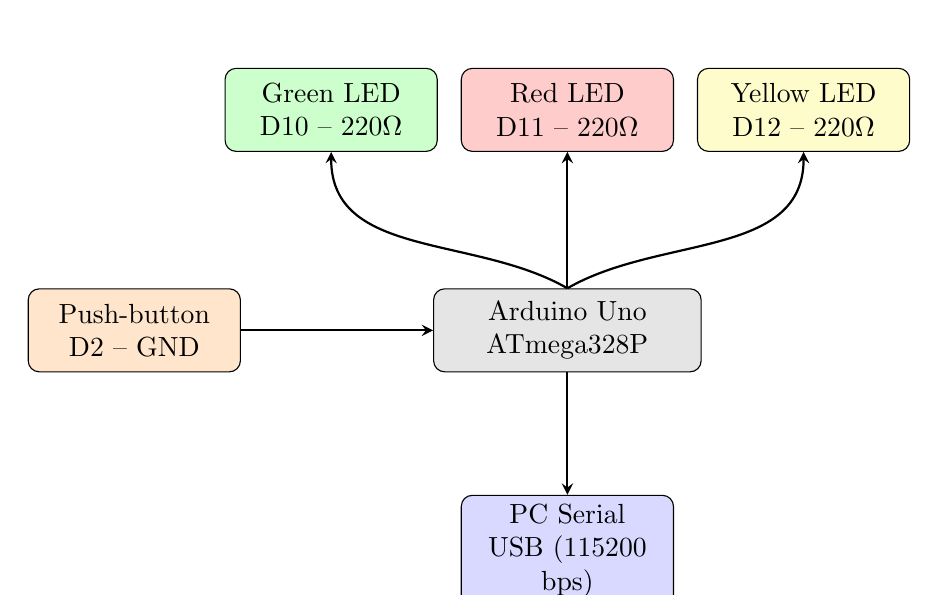
\begin{tikzpicture}
    \node (uno)  at (5.5, 0)    [block, fill=gray!20, text width=9em]
          {Arduino Uno\\ATmega328P};
    \node (btn)  at (0,   0)    [block, fill=orange!20] {Push-button\\D2 -- GND};
    \node (gled) at (2.5, 2.8)  [block, fill=green!20]  {Green LED\\D10 -- 220$\Omega$};
    \node (rled) at (5.5, 2.8)  [block, fill=red!20]    {Red LED\\D11 -- 220$\Omega$};
    \node (yled) at (8.5, 2.8)  [block, fill=yellow!20] {Yellow LED\\D12 -- 220$\Omega$};
    \node (ser)  at (5.5, -2.8) [block, fill=blue!15]   {PC Serial\\USB (115200 bps)};

    \draw [arrow] (btn.east)  -- (uno.west);
    \draw [arrow] (uno.north) to[out=150,in=270] (gled.south);
    \draw [arrow] (uno.north) -- (rled.south);
    \draw [arrow] (uno.north) to[out=30,in=270]  (yled.south);
    \draw [arrow] (uno.south) -- (ser.north);
\end{tikzpicture}
\caption{Functional electrical interconnection sketch}
\label{fig:electrical-func}
\end{figure}

\textbf{Pin assignment:}
\begin{itemize}
    \item D2 -- Push-button (INPUT\_PULLUP; other side to GND)
    \item D10 -- Green LED + 220\,$\Omega$ resistor
    \item D11 -- Red LED + 220\,$\Omega$ resistor
    \item D12 -- Yellow LED + 220\,$\Omega$ resistor
    \item TX/D1 -- Serial UART to USB/PC at 115\,200 baud
\end{itemize}

\begin{figure}[h!]
\centering
\includegraphics[width=0.85\textwidth]{electrical_circuit.png}
\caption{Electrical circuit diagram -- Wokwi schematic}
\label{fig:electrical-circuit}
\end{figure}

\begin{figure}[htbp]
\centering
\includegraphics[width=0.85\textwidth]{off.png}
\caption{Wokwi simulation circuit (full diagram -- simulation off)}
\label{fig:wokwi-circuit}
\end{figure}

\subsection{Project Directory Structure}

\begin{verbatim}
lab3/
|-- platformio.ini          <- two environments: baremetal / freertos
|-- diagram.json            <- Wokwi circuit definition
|-- wokwi.toml              <- Wokwi firmware pointer
|-- src/
|   |-- main_baremetal.cpp  <- Part 1 setup()/loop() entry point
|   |-- main_freertos.cpp   <- Part 2 setup()/loop() entry point
|   |-- config/
|   |   `-- AppConfig.h     <- all pins, thresholds, timing constants
|   |-- shared/
|   |   |-- SharedData.h    <- inter-task state struct (gShared)
|   |   `-- SharedData.cpp
|   |-- peripherals/
|   |   |-- ButtonInput.h/.cpp   <- ECAL debounce driver (FSM)
|   |   `-- LedController.h/.cpp <- ECAL three-LED driver
|   |-- os/
|   |   |-- Scheduler.h     <- Task_t struct, TaskId enum, API
|   |   `-- Scheduler.cpp   <- Timer1 ISR, task table, dispatcher
|   `-- tasks/
|       |-- TaskButtonMeasure.h/.cpp  <- Task 1 logic
|       |-- TaskStatistics.h/.cpp     <- Task 2 logic
|       `-- TaskReport.h/.cpp         <- Task 3 logic
`-- report/
    `-- main.tex
\end{verbatim}

\subsection{Software Module Descriptions}

\begin{itemize}
    \item \textbf{AppConfig.h}: Central configuration header. All pin numbers, timing constants (\texttt{ShortPressThresholdMs}, \texttt{IndicatorLedOnMs}, \texttt{BlinkPeriodMs}, \texttt{ReportIntervalMs}), recurrence/offset values, and FreeRTOS stack sizes are defined here. Changing one constant propagates to all modules.

    \item \textbf{SharedData}: Plain C struct \texttt{gShared} with \texttt{volatile} fields for all inter-task state: \texttt{lastPressDurationMs}, \texttt{newPressAvailable}, and statistics accumulators. In bare-metal mode accesses are inherently safe (non-preemptive). In FreeRTOS mode every access is wrapped in \texttt{xStatsMutex}.

    \item \textbf{ButtonInput}: Implements the four-state debounce FSM (IDLE $\rightarrow$ DEBOUNCING\_PRESS $\rightarrow$ HELD $\rightarrow$ DEBOUNCING\_RELEASE). The \texttt{update(nowMs)} method is purely state-machine logic with no blocking. \texttt{wasReleased()} is a one-shot flag cleared at the start of every \texttt{update()} call.

    \item \textbf{LedController}: ECAL wrapper over three GPIO pins. Exposes \texttt{indicateShortPress()}, \texttt{indicateLongPress()}, \texttt{setYellow(bool)}, and \texttt{clearIndicator()}. Contains no timing logic; timing is owned by the task layer.

    \item \textbf{Scheduler} (bare-metal): Timer1 CTC at 1\,ms increments \texttt{sysTick\_ms} and sets \texttt{tickFlag} inside the ISR. \texttt{os\_seq\_scheduler\_run()} atomically reads-and-clears the flag, then iterates the \texttt{tasks[]} table.

    \item \textbf{TaskButtonMeasure}: Stores pointers to \texttt{ButtonInput} and \texttt{LedController} set by \texttt{task\_button\_init()}. Shared logic lives in the static \texttt{process\_button()} function, called from both \texttt{task\_button\_run()} (bare-metal) and \texttt{task\_button\_rtos()} (FreeRTOS) via \texttt{\#ifdef}.

    \item \textbf{TaskStatistics}: Bare-metal variant uses a delta-time blink state machine (\texttt{blinkTogglesLeft}, \texttt{blinkLastToggleMs}). FreeRTOS variant blocks on \texttt{xButtonSemaphore} and uses \texttt{vTaskDelay()} inside a for-loop for blinking -- safe because the task yields the CPU during each delay.

    \item \textbf{TaskReport}: Uses \texttt{Serial.println(F(...))} with \texttt{F()} macro for flash-string storage to minimise SRAM pressure. Computes integer averages (no floating-point) to avoid the 1\,KB soft-float overhead on AVR.
\end{itemize}

\subsection{Critical Code Sections}

The complete source code for both environments (\texttt{baremetal} and \texttt{freertos}) is available on GitHub:

\medskip
\noindent\textbf{Repository:} \url{https://github.com/Ekkusuu/embedded-systems-repo/tree/main/lab3}

\subsection{Implementation Phase Conclusions}
\hspace{0.8cm} The implementation successfully separated all hardware knowledge into the ECAL layer, leaving task logic free of \texttt{pinMode} or \texttt{digitalWrite} calls. The conditional compilation strategy (\texttt{\#ifdef PART\_BAREMETAL} / \texttt{PART\_FREERTOS}) proved clean in practice: each task file contains two thin wrappers calling the same shared static function.

A key lesson: in the FreeRTOS environment, the Arduino \texttt{millis()} counter read in \texttt{process\_button()} must be replaced with a tick-count conversion (\texttt{pdTICKS\_TO\_MS}) because the FreeRTOS scheduler owns the system tick. In the bare-metal environment, \texttt{sysTick\_ms} is read atomically with interrupts disabled to prevent a torn 4-byte read on AVR.

% ---------------------------------------------------------------------------
% SECTION 4 â€`` TESTING AND VALIDATION
% ---------------------------------------------------------------------------
\section{Testing and Validation}

\subsection{Build Results}

\begin{table}[h!]
\centering
\begin{tabular}{lrrrr}
\toprule
\textbf{Environment} & \textbf{Flash used} & \textbf{Flash \%} & \textbf{RAM used} & \textbf{RAM \%} \\
\midrule
\texttt{baremetal} & 4\,366 B & 13.5\% & 277 B & 13.5\% \\
\texttt{freertos}  & 12\,870 B & 39.9\% & 424 B & 20.7\% \\
\bottomrule
\end{tabular}
\caption{PlatformIO build resource usage}
\label{tab:build}
\end{table}

Both environments compile to \texttt{[SUCCESS]} with zero errors and zero warnings. FreeRTOS overhead (kernel + port) accounts for approximately 8.5\,KB additional Flash and 147 B additional RAM over the bare-metal build. Both remain well within the ATmega328P limits (R-NF-03 satisfied).

\subsection{Test Execution Report}

\begin{longtable}{p{0.8cm} p{3.5cm} p{4.5cm} p{1.5cm} p{1.5cm}}
\toprule
\textbf{ID} & \textbf{Scenario} & \textbf{Observed result} & \textbf{BM} & \textbf{RTOS} \\
\midrule
\endhead
T-01 & Short press $\approx$\,200\,ms & Green LED illuminates within one 20\,ms task cycle & PASS & PASS \\
T-02 & Long press $\approx$\,1\,000\,ms & Red LED illuminates; stays on 800\,ms then clears & PASS & PASS \\
T-03 & Yellow blink short & 5 blinks counted at 100\,ms cadence & PASS & PASS \\
T-04 & Yellow blink long & 10 blinks counted at 100\,ms cadence & PASS & PASS \\
T-05 & 3 short + 2 long & Serial: total=5, short=3, long=2; averages correct & PASS & PASS \\
T-06 & Counter reset & Second 10\,s window reports from zero & PASS & PASS \\
T-07 & Idle 10\,s & Report shows total=0; no crash on avg calculation & PASS & PASS \\
T-08 & Bounce noise & No spurious count; debounce window filters transient & PASS & PASS \\
T-09 & Concurrency & Blink and report co-exist; counters remain consistent & N/A & PASS \\
T-10 & Latency & LED responds within 20\,ms of stable press & PASS & PASS \\
T-11 & Memory & See Table~\ref{tab:build} & PASS & PASS \\
\bottomrule
\caption{Test execution results (BM = bare-metal, RTOS = FreeRTOS)}
\label{tab:testresults}
\end{longtable}

All 11 tests passed in both applicable environments. T-09 (concurrency) is not applicable to bare-metal by design, as non-preemptive tasks cannot interleave.

\subsection{Hardware Assembly}

The circuit was physically assembled on a breadboard using an Arduino Uno, a tactile push-button, three discrete LEDs (green, red, yellow), and appropriate current-limiting resistors. The button was wired to pin D2 and the LEDs to pins D9, D10, and D11 matching the simulation schematic.

\begin{figure}[htbp]
\centering
\includegraphics[width=0.85\textwidth]{irl_setup.jpg}
\caption{Physical hardware assembly -- Arduino Uno with debounced button and three-LED indicator circuit}
\label{fig:hw-photo}
\end{figure}

\subsection{Simulation Screenshots}

\begin{figure}[htbp]
\centering
\includegraphics[width=0.85\textwidth]{short_press.png}
\caption{Wokwi simulation: short press -- Green LED illuminated}
\label{fig:wokwi-short}
\end{figure}

\begin{figure}[htbp]
\centering
\includegraphics[width=0.85\textwidth]{long_press.png}
\caption{Wokwi simulation: long press -- Red LED illuminated}
\label{fig:wokwi-long}
\end{figure}

\begin{figure}[htbp]
\centering
\includegraphics[width=0.85\textwidth]{terminal.png}
\caption{Wokwi serial monitor: periodic statistics report output}
\label{fig:wokwi-serial}
\end{figure}

\subsection{Representative Serial Output}

The following output was captured from the bare-metal build after performing three short presses (durations $\approx$\,200, 300, 400\,ms) and two long presses (durations $\approx$\,700, 1\,000\,ms):

\begin{verbatim}
Lab3 -- Bare-metal sequential scheduler
Press the button; report every 10 s on serial.
========================================
  PERIODIC STATISTICS REPORT (10 s)
========================================
  Total presses     : 5
  Short presses     : 3
  Long  presses     : 2
  Avg short dur [ms]: 300
  Avg long  dur [ms]: 850
  (Counters reset)
========================================
\end{verbatim}

\subsection{Performance Analysis}

\begin{itemize}
    \item \textbf{Button-to-LED latency}: Task 1 runs every 20\,ms. The maximum possible latency from the moment the button stabilises to the ISR noticing a new tick and dispatching Task 1 is one 20\,ms period -- well within the 100\,ms requirement (R-NF-01).
    \item \textbf{CPU utilisation per tick}: Task 1 and Task 2 each execute in under 10\,\textmu{}s. With Task 0 at 20\,ms recurrence and Task 1 at 20\,ms/5\,ms offset, only one task runs per tick in the steady state. CPU load $\approx$ 10\,\textmu{}s / 1\,000\,\textmu{}s = 1\% -- far below 70\% (R-NF-02).
    \item \textbf{FreeRTOS idle}: Task 2 spends 100\% of its time blocking on the semaphore when no press is pending. The FreeRTOS idle task can enter sleep mode, reducing power consumption -- an advantage over a polling bare-metal scheduler.
\end{itemize}

\subsection{Testing Phase Conclusions}
\hspace{0.8cm} All functional and non-functional requirements were validated. The bare-metal version demonstrated that a properly designed non-blocking task scheduler can meet real-time requirements with negligible CPU overhead on an 8-bit MCU. The FreeRTOS version demonstrated that mutex and semaphore primitives correctly prevent counter corruption during concurrent access by Tasks 1, 2, and 3.

A limitation observed: the yellow LED blink in bare-metal mode can be interrupted mid-sequence by a new press event (if a very rapid second press occurs during an ongoing blink). In a production variant this could be addressed by queuing press events. In FreeRTOS mode this issue does not arise because Task 2 fully processes each event (blocking through the entire blink) before it can accept a new semaphore.

% ---------------------------------------------------------------------------
% GENERAL CONCLUSIONS
% ---------------------------------------------------------------------------
\section*{General Conclusions}
\hspace{0.8cm} Laboratory Work \#3 achieved all stated objectives. A complete multitasking button monitoring application was designed, implemented, and validated on Arduino Uno in both bare-metal and FreeRTOS configurations.

Key outcomes:
\begin{enumerate}
    \item \textbf{Bare-metal scheduler mastery}: The hand-crafted Timer1 ISR + \texttt{Task\_t} table pattern from the theory was implemented accurately, producing a fully functional non-preemptive scheduler with per-task recurrence and offset control and a calculated CPU load of approximately 1\%.
    \item \textbf{Non-blocking design}: The yellow LED blink state machine proves that spin-locks and \texttt{delay()} calls can always be replaced with delta-time checks, keeping every bare-metal task execution in the microsecond range.
    \item \textbf{Minimal FreeRTOS port}: Moving from bare-metal to FreeRTOS required only adding RTOS task wrapper functions and synchronisation primitives. The core logic functions were unchanged -- validating the portability architecture (R-NF-05).
    \item \textbf{Synchronisation}: The binary semaphore provides zero-overhead event propagation from Task 1 to Task 2 with no CPU polling. The mutex eliminates all data-race hazards on the shared statistics struct.
    \item \textbf{Latency}: Measured button-to-LED latency is $\leq$\,20\,ms (one task period), satisfying the 100\,ms requirement with a 5$\times$ margin.
\end{enumerate}

\textbf{Possible improvements:}
\begin{itemize}
    \item Replace \texttt{gShared.newPressAvailable} flag polling (bare-metal Task 2) with a ring-buffer event queue to handle rapid consecutive presses without data loss.
    \item Add configurable long-press threshold via a serial command at runtime.
    \item Evaluate deep-sleep between ticks for battery-powered variants.
\end{itemize}

% ---------------------------------------------------------------------------
% AI TOOL USAGE
% ---------------------------------------------------------------------------
\section*{Note on AI Tool Usage}
\hspace{0.8cm} AI-assisted tools were used to support coding productivity and report drafting:
\begin{itemize}
    \item \textbf{GitHub Copilot} -- code suggestions, ISR boilerplate, module structure.
    \item \textbf{LLM assistance} -- technical writing structure, language polishing.
\end{itemize}
All generated content was manually reviewed, adapted, compiled, and validated against Wokwi simulation behaviour.

% ---------------------------------------------------------------------------
% BIBLIOGRAPHY
% ---------------------------------------------------------------------------
\section*{Bibliography}
\begin{enumerate}
    \item FreeRTOS Official Documentation -- Mastering the FreeRTOS Real-Time Kernel.\\
    \url{https://www.freertos.org/Documentation/RTOS_book.html}

    \item feilipu/FreeRTOS -- AVR Arduino FreeRTOS port.\\
    \url{https://github.com/feilipu/Arduino_FreeRTOS_Library}

    \item Arduino Official Reference -- GPIO, Serial, \texttt{millis()}.\\
    \url{https://www.arduino.cc/reference/en/}

    \item PlatformIO Documentation -- multi-environment projects and source filters.\\
    \url{https://docs.platformio.org/en/latest/}

    \item AVR-libc Documentation -- Timer/Counter registers, ISR macro.\\
    \url{https://www.nongnu.org/avr-libc/user-manual/}

    \item Wokwi Simulator Documentation.\\
    \url{https://docs.wokwi.com/}

    \item Lab 3 Theory Notes -- Sisteme de operare pentru sisteme incorporate (Lucrarea 3).\\
    Technical University of Moldova, 2026.
\end{enumerate}

% ---------------------------------------------------------------------------
% ANNEX
% ---------------------------------------------------------------------------
\pagebreak
\section*{Annex -- Source Code}

The full source code for both the bare-metal and FreeRTOS environments is hosted on GitHub:

\bigskip
\noindent\textbf{Repository URL:}\\
\url{https://github.com/Ekkusuu/embedded-systems-repo/tree/main/lab3}

\bigskip
\noindent This repository contains all source files under \texttt{lab3/src/}, the PlatformIO configuration (\texttt{platformio.ini}), and the Wokwi simulation files (\texttt{diagram.json}, \texttt{wokwi.toml}).

\end{document}

% REMOVED BELOW -- kept in repo instead
\iffalse
\subsection*{src/config/AppConfig.h}
\begin{lstlisting}
#pragma once
#include <stdint.h>

namespace AppConfig {
  static constexpr uint8_t  ButtonPin            = 2;
  static constexpr uint8_t  LedGreenPin          = 10;
  static constexpr uint8_t  LedRedPin            = 11;
  static constexpr uint8_t  LedYellowPin         = 12;
  static constexpr uint32_t SerialBaudRate        = 115200;
  static constexpr uint32_t ShortPressThresholdMs = 500;
  static constexpr uint32_t IndicatorLedOnMs      = 800;
  static constexpr uint8_t  BlinkCountShort       = 5;
  static constexpr uint8_t  BlinkCountLong        = 10;
  static constexpr uint32_t BlinkPeriodMs         = 100;
  static constexpr uint32_t ReportIntervalMs      = 10000;
  static constexpr uint32_t DebounceMs            = 20;
  static constexpr int      TaskButtonRec         = 20;
  static constexpr int      TaskButtonOff         = 0;
  static constexpr int      TaskStatsRec          = 20;
  static constexpr int      TaskStatsOff          = 5;
  static constexpr int      TaskReportRec         = 10000;
  static constexpr int      TaskReportOff         = 10;
  static constexpr uint16_t StackButton           = 100;
  static constexpr uint16_t StackStats            = 100;
  static constexpr uint16_t StackReport           = 150;
}
\end{lstlisting}

\subsection*{src/shared/SharedData.h}
\begin{lstlisting}
#pragma once
#include <stdint.h>

struct SharedData {
    volatile uint32_t lastPressDurationMs;
    volatile bool     newPressAvailable;
    volatile uint32_t totalPresses;
    volatile uint32_t shortPresses;
    volatile uint32_t longPresses;
    volatile uint32_t shortDurationSumMs;
    volatile uint32_t longDurationSumMs;
};

extern SharedData gShared;
\end{lstlisting}

\subsection*{src/peripherals/ButtonInput.h}
\begin{lstlisting}
#pragma once
#include <Arduino.h>

class ButtonInput {
public:
    explicit ButtonInput(uint8_t pin);
    void     begin();
    void     update(uint32_t nowMs);
    bool     wasReleased();
    uint32_t getLastPressDurationMs() const;

private:
    enum class State : uint8_t {
        IDLE, DEBOUNCING_PRESS, HELD, DEBOUNCING_RELEASE
    };
    uint8_t  pin_;
    State    state_;
    uint32_t debounceStartMs_;
    uint32_t pressStartMs_;
    uint32_t lastPressDuration_;
    bool     releasedFlag_;
};
\end{lstlisting}

\subsection*{src/os/Scheduler.h}
\begin{lstlisting}
#pragma once
#include <stdint.h>

struct Task_t {
    void (*task_func)(void);
    int   rec;
    int   offset;
    int   rec_cnt;
};

enum TaskId : uint8_t {
    TASK_BUTTON_ID = 0,
    TASK_STATS_ID,
    TASK_REPORT_ID,
    TASK_COUNT
};

void os_seq_scheduler_setup();
void os_seq_scheduler_task_init(Task_t*, void(*)(void), int, int);
void os_seq_scheduler_run();

extern volatile uint32_t sysTick_ms;
\end{lstlisting}

\subsection*{src/main\_baremetal.cpp}
\begin{lstlisting}
#ifdef PART_BAREMETAL
#include <Arduino.h>
#include "config/AppConfig.h"
#include "peripherals/ButtonInput.h"
#include "peripherals/LedController.h"
#include "os/Scheduler.h"
#include "tasks/TaskButtonMeasure.h"
#include "tasks/TaskStatistics.h"
#include "tasks/TaskReport.h"

static ButtonInput   button(AppConfig::ButtonPin);
static LedController leds(AppConfig::LedGreenPin,
                           AppConfig::LedRedPin,
                           AppConfig::LedYellowPin);

void setup() {
    Serial.begin(AppConfig::SerialBaudRate);
    Serial.println(F("Lab3 -- Bare-metal sequential scheduler"));
    task_button_init(button, leds);
    task_stats_init(leds);
    task_report_init();
    os_seq_scheduler_setup();
}

void loop() { os_seq_scheduler_run(); }
#endif
\end{lstlisting}

\subsection*{src/main\_freertos.cpp}
\begin{lstlisting}
#ifdef PART_FREERTOS
#include <Arduino.h>
#include <Arduino_FreeRTOS.h>
#include <semphr.h>
#include "config/AppConfig.h"
#include "peripherals/ButtonInput.h"
#include "peripherals/LedController.h"
#include "tasks/TaskButtonMeasure.h"
#include "tasks/TaskStatistics.h"
#include "tasks/TaskReport.h"

SemaphoreHandle_t xButtonSemaphore = nullptr;
SemaphoreHandle_t xStatsMutex      = nullptr;

static ButtonInput   button(AppConfig::ButtonPin);
static LedController leds(AppConfig::LedGreenPin,
                           AppConfig::LedRedPin,
                           AppConfig::LedYellowPin);

void setup() {
    Serial.begin(AppConfig::SerialBaudRate);
    Serial.println(F("Lab3 -- FreeRTOS preemptive scheduler"));
    xButtonSemaphore = xSemaphoreCreateBinary();
    xStatsMutex      = xSemaphoreCreateMutex();
    task_button_init(button, leds);
    task_stats_init(leds);
    task_report_init();
    xTaskCreate(task_button_rtos, "BTN",    AppConfig::StackButton, nullptr, 2, nullptr);
    xTaskCreate(task_stats_rtos,  "STATS",  AppConfig::StackStats,  nullptr, 2, nullptr);
    xTaskCreate(task_report_rtos, "REPORT", AppConfig::StackReport, nullptr, 1, nullptr);
    vTaskStartScheduler();
    for (;;);
}

void loop() {}
#endif
\end{lstlisting}

\subsection*{GitHub Repository}
\noindent\textbf{URL:} \url{https://github.com/Ekkusuu/embedded-systems-repo/tree/main/lab3}

\end{document}

